\chapter{Experiments\label{chap:experiments}}

This chapter discusses the various experiments conducted on the dataset and their results. We will first go through techniques used to train various models and then the metrics used to compare the results.

\section{Training Experiments}

As mentioned in Chapter \ref{chap:dataset}, we don't have a balanced dataset. The number of malware samples are much greater than the benign samples. Due to this, we use cross-validation technique to train and test our machine learning models on our imbalanced dataset.

\subsection{Cross-Validation}

Cross-validation is a technique to evaluate how machine learning models perform on the given dataset. It is mainly used in situations such as ours where there is not enough data to divide the dataset into separate training and testing sets. Cross validation can be divided into two types:

\begin{itemize}
	\item Exhaustive cross-validation:
	In this cross-validation method we learn and test on all possible combinations of the training and testing dataset.
	\begin{itemize}
		\item Leave-\emph{p}-out:
		Leave-\emph{p}-out is a type of exhaustive cross-validation where we use \emph{p} sets as validation set and the remaining are used as training set.
	\end{itemize}
	\item Non-exhaustive cross-validation:
	In this cross-validation method we do not compute all possible combinations of the training and testing dataset.
	\begin{itemize}
		\item Holdout method:
		This is the simplest cross-validation method where the dataset is separated into two sets, the training and testing set.
		\item \emph{k}-fold cross-validation:
		In this cross-validation method we divide the dataset into \emph{k} subsets and then the model is iteratively tested on one set and trained on the remaining set.
	\end{itemize}
\end{itemize}

We use 10-fold cross-validation in all our experiments. As shown in Figure \ref{fig:10-fold}, our dataset is divided into ten subsets and the model is then iteratively trained on nine subsets and tested on one subset.

\begin{figure}[htb]
	\centering
	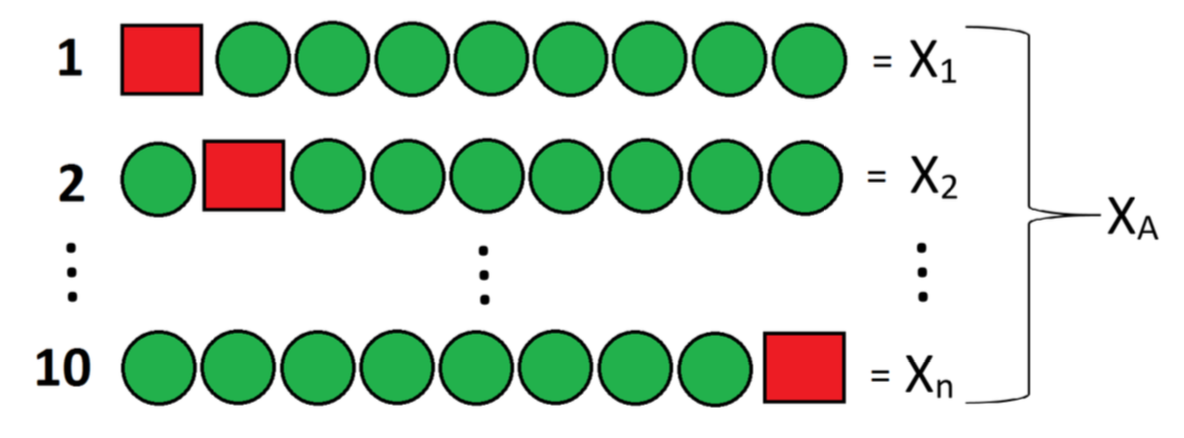
\includegraphics[width=0.7\textwidth]{images/k-fold.png}
	\caption{10-fold cross-validation. The red rectangle is the testing set and the other subsets are used for training.} 
	\label{fig:10-fold}
\end{figure}

\section{Evaluation Metrics}

We use \emph{accuracy} as our evaluation method for all the experiments. \emph{Accuracy} is used to measure how well the model could detect malicious network traffic among the dataset. \emph{Accuracy} can be defined as:
$$
Accuracy = \dfrac{TP + TN}{ TP + TN + FP + FN}
$$
\emph{where},
\begin{align*}
	TP: True\;Positives \\
	TN: True\;Negatives\\
	FP: False\;Positives\\
	FN: False\;Negatives\\
\end{align*}

\section{Data Analysis}

As we can see from Figure \ref{fig:orig-port-freq}, in the initial data analysis, we found that the most frequent ports in malware captures are different than the most frequent ports in benign captures. We can see a similar result in Figure \ref{fig:resp-port-freq} where we plot the frequency of ports used by the responding endpoint in the network traffic capture. The top 5 ports with most frequency in both the captures are shown in Table \ref{tab:3}.

\begin{figure}[htb]
	\centering
	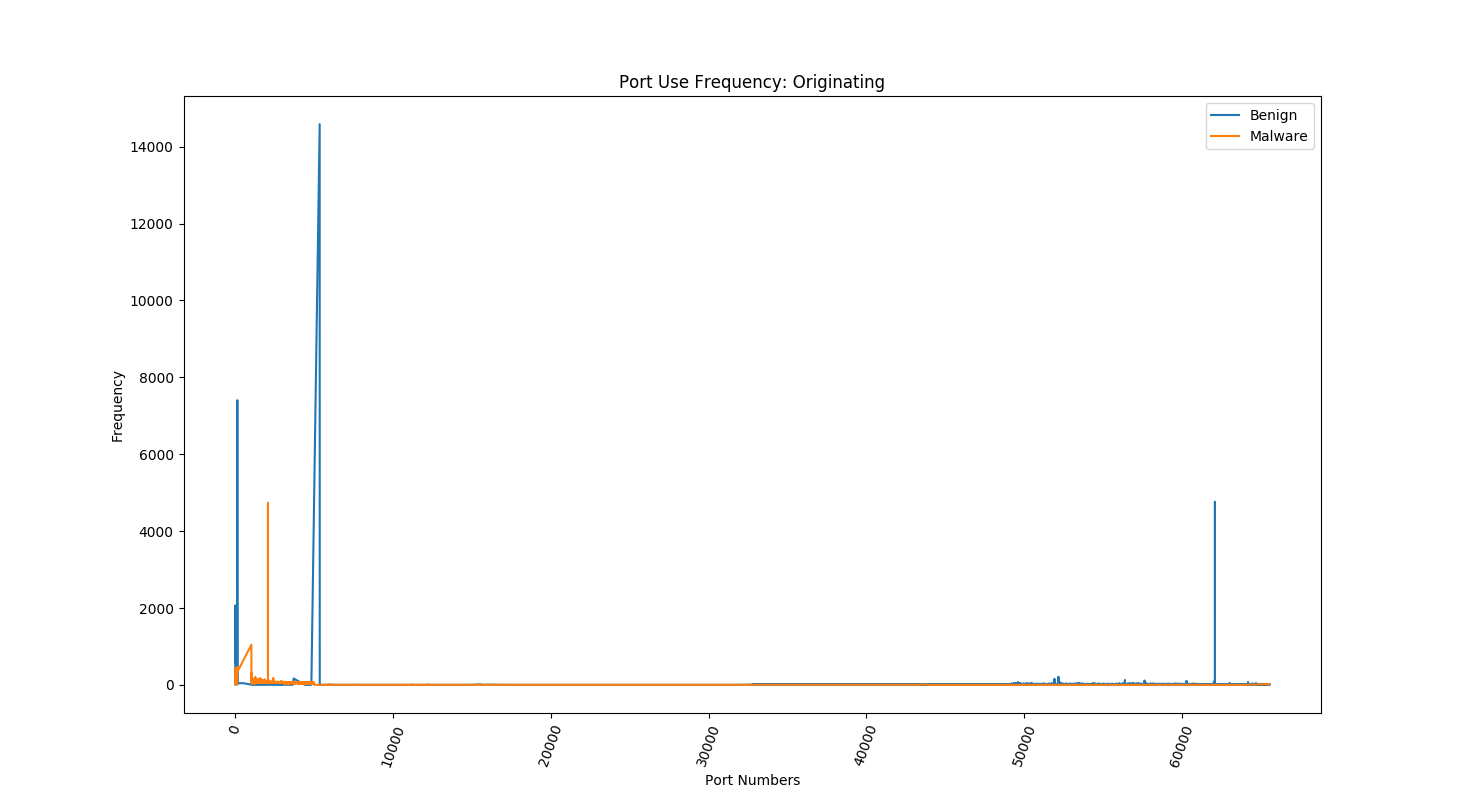
\includegraphics[width=1\textwidth]{images/orig-port-freq.png}
	\caption{Frequency of ports used by ORIG} 
	\label{fig:orig-port-freq}
\end{figure}

\begin{figure}[htb]
	\centering
	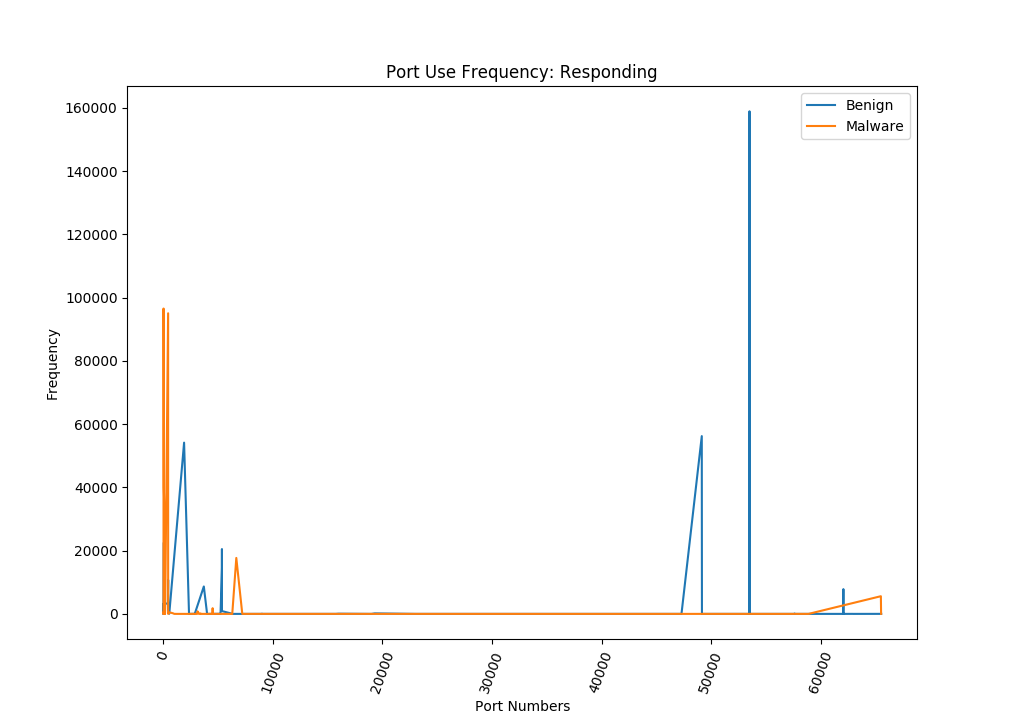
\includegraphics[width=1\textwidth]{images/resp-port-freq.png}
	\caption{Frequency of ports used by RESP} 
	\label{fig:resp-port-freq}
\end{figure}

\begin{table}[!htb]
	\caption{Top Five Ports Used by ORIG\label{tab:3}}
	\begin{center}
		\begin{tabular}{c|p{0.15\textwidth}|p{0.50\textwidth}}\hline\hline
			Dataset & Port Number & \multicolumn{1}{l}{Known Port Assignments} \\ \hline
			Malware & 2077 & WebDisk or Old Tivoli Storage \\
			& 2079	&  IDWARE Router Port\\
			& 1025	&  Ports > 1024 are designated for dynamic allocation by Windows\\
			& 137	&  File and Print Sharing under Windows\\
			& 3 &  Compression Process \\ \hline
			Benign & 5353  &  Multicast DNS, iChat, Mac OS X Bonjour\\
			& 135 &  Remote Procedure Call (RPC)\\
			& 62078 &  UPnP (Universal Plug and Play), iTunes\\
			& 137 &  File and Print Sharing under Windows\\
			& 138 &  File and Print Sharing under Windows\\
			\hline\hline
		\end{tabular}
	\end{center}
\end{table}

\begin{table}[!htb]
	\caption{Top Five Ports Used by RESP\label{tab:4}}
	\begin{center}
		\begin{tabular}{c|p{0.15\textwidth}|p{0.50\textwidth}}\hline\hline
			Dataset & Port Number & \multicolumn{1}{l}{Known Port Assignments} \\ \hline
			Malware & 25 & SMTP (Simple Mail Transfer Protocol) \\
			& 443	&  HTTPS / SSL - encrypted web traffic\\
			& 53	&  DNS (Domain Name Service)\\
			& 80	&  Hyper Text Transfer Protocol (HTTP) \\
			& 6667 &  IRC (Internet Relay Chat) \\ \hline
			Benign & 53508  &  Xsan Filesystem Apple\\
			& 49153 &  ANTLR, ANother Tool for Language Recognition\\
			& 1900 &  IANA registered by Microsoft for SSDP (Simple Service Discovery Protocol)\\
			& 53 &  DNS (Domain Name Service)\\
			& 5355 &  Link-Local Multicast Name Resolution Windows\\
			\hline\hline
		\end{tabular}
	\end{center}
\end{table}

As we can see from Table \ref{tab:3} and Table \ref{tab:4}, malware dataset had Internet Relay Chat (IRC) port among the most frequently used. We know that most of the malware use IRC to exfiltrate data from the infected system to other systems. We also see that HTTPS port 443 is also among the most frequently used in the malware captures.

\section{K-means Clustering}

K-means clustering is an unsupervised learning algorithm that aims to partition \verb|n| data points into \verb|k| clusters. Clustering is used to see whether the data points naturally form distinct clusters or whether they are similar to other data points in the dataset. We normalized the values in our dataset and performed K-means clustering with \verb|k=2|. The results are shown in the following figures:

\begin{figure}[htb]
	\centering
	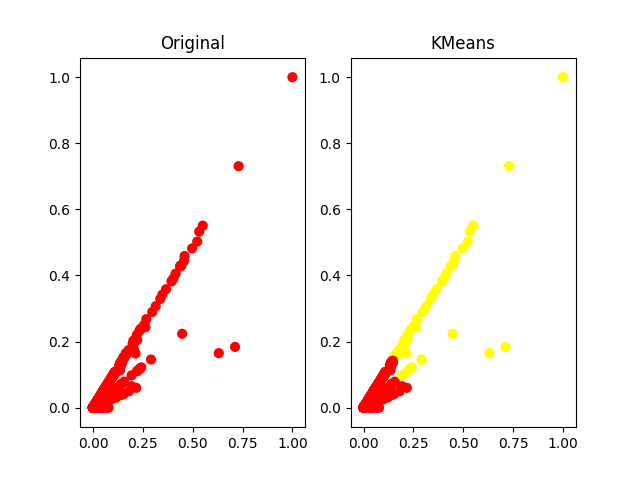
\includegraphics[width=1\textwidth]{images/kmeans.png}
	\caption{Original Scatter Plot vs K-means clustering} 
	\label{fig:kmeans1}
	
	\centering
	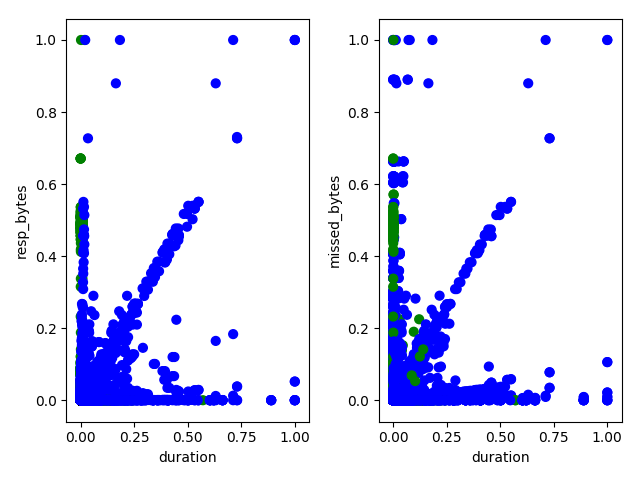
\includegraphics[width=1\textwidth]{images/kmeans2.png}
	\caption{Original Scatter Plots with different axes} 
	\label{fig:kmeans2}
\end{figure}

As seen in Figure \ref{fig:kmeans1}, K-means didn't really give us distinct clusters. Also , the most of the scatter plots based on connection features resemble that in Figure \ref{fig:kmeans2}. We can further perform experiments such as Support Vector Machine (SVM) to find prominent features in the dataset.

\clearpage

\section{Experiments}

We performed multiple experiments using different machine learning techniques.

\subsection{Experiment 1}

In this experiment we ran SVM with linear kernel with 10-fold cross validation on our dataset and achieved an average \emph{Accuracy rate} of $92.07$\% as shown in Figure \ref{fig:result_svm}.

\begin{figure}[htb]
	\centering
	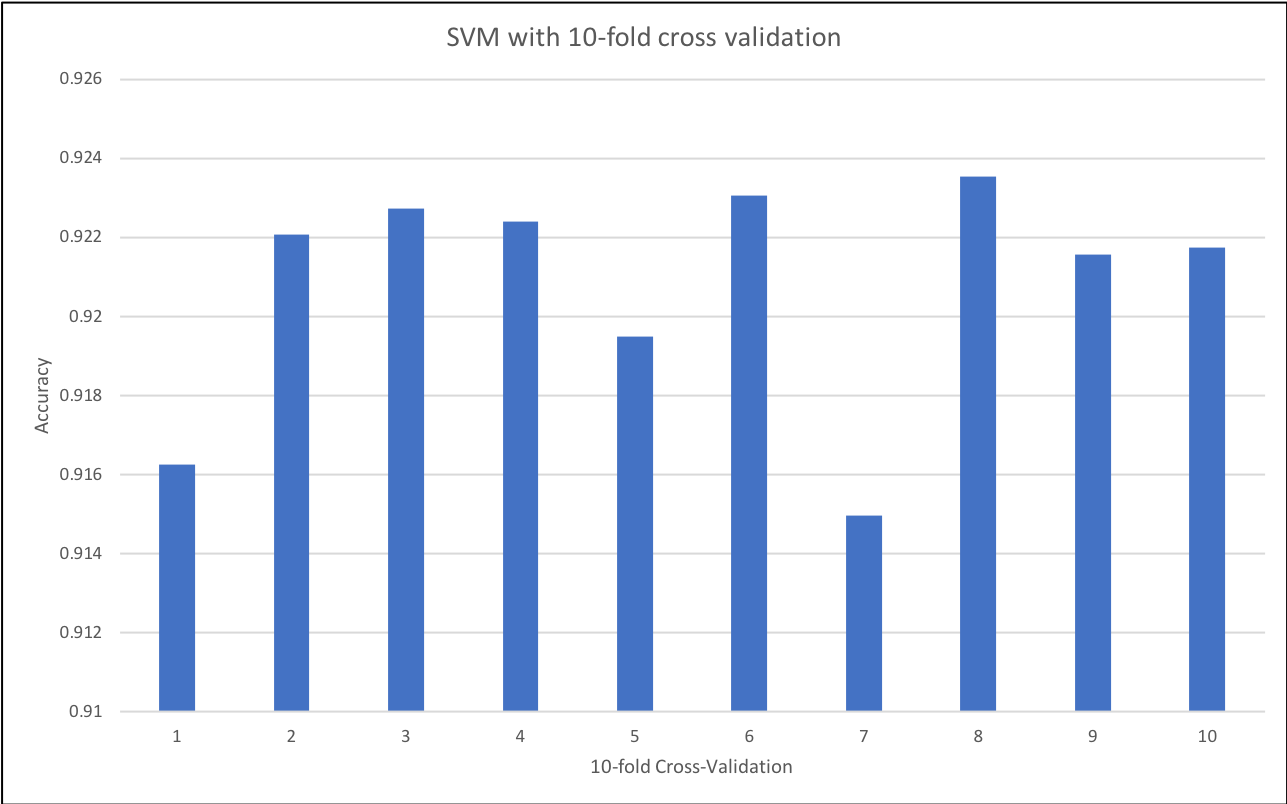
\includegraphics[width=0.7\textwidth]{images/svm.png}
	\caption{SVM with 10-fold cross-validation} 
	\label{fig:result_svm}
\end{figure}

SVM also assigns weights to the input features which gave us an insight into the features SVM believes are important. In Figure \ref{fig:result_svm_weights}, we can see that SVM assigned the highest weight to feature number 16. The rank assigned to each feature can be seen in Table \ref{tab:5}. We can see that average certificate length, periodicity and average public key length are the top most features. Also from \cite{AndersonM16} we know that malware use weak encryption techniques such as shorter key lengths and are more periodic in nature than other applications. Also, the validity of certificate during capture is the sixth highest rank feature which tell us that most of malware may not have a valid certificate.

 \begin{figure}[htb]
 	\centering
 	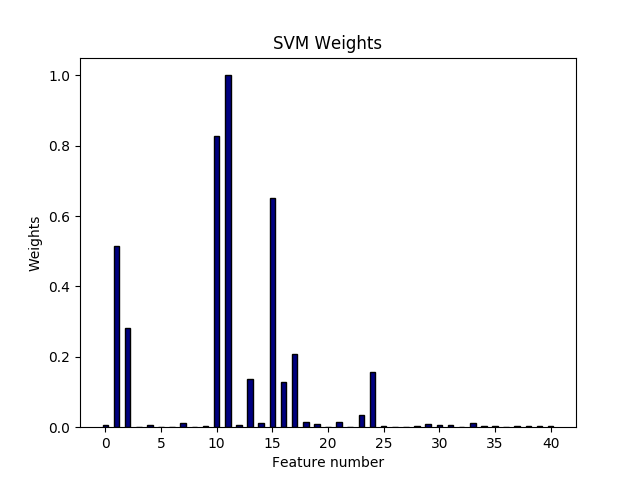
\includegraphics[width=0.7\textwidth]{images/svm_weights.png}
 	\caption{SVM assigned weights to the features} 
 	\label{fig:result_svm_weights}
 \end{figure}

\begin{table}[!htb]
	\caption{Feature Ranks by SVM (Highest Ranked First) \label{tab:5}}
	\begin{center}
		\begin{tabular}{c|p{0.50\textwidth}}\hline\hline
			Rank & Feature  \\ \hline
			 1  & average\_of\_certificate\_length           \\
			 2  & periodicity\_standard\_deviation           \\
			 3  & periodicity\_average                       \\
			 4  & standart\_deviation\_cert\_length          \\
			 5  & average\_public\_key                       \\
			 6  & is\_valid\_certificate\_during\_capture    \\
			 7  & average\_of\_duration                      \\
			 8  & standard\_deviation\_duration              \\
			 9  & self\_signed\_ratio                        \\
			 10 & SNI\_ssl\_ratio                            \\
			 11 & ratio\_of\_differ\_sandns\_in\_cert        \\
			 12 & percent\_of\_established\_states           \\
			 13 & number\_of\_certificate\_path              \\
			 14 & ratio\_of\_differ\_subject\_in\_cert       \\
			 15 & ratio\_of\_differ\_subject\_in\_ssl\_log   \\
			 16 & tls\_version\_ratio                        \\
			 17 & is\_SNI\_in\_top\_level\_domain            \\
			 18 & total\_size\_of\_flows\_orig               \\
			 19 & ratio\_of\_sizes                           \\
			 20 & ratio\_of\_differ\_issuer\_in\_ssl\_log    \\
			 21 & ratio\_of\_same\_subjects                  \\
			 22 & ratio\_of\_same\_issuer                    \\
			 23 & average\_certificate\_exponent             \\
			 24 & outbound\_pckts                            \\
			 25 & number\_of\_flows                          \\
			 26 & is\_SNIs\_in\_SNA\_dns                     \\
			 27 & ratio\_certificate\_path\_error            \\
			 28 & ratio\_missing\_cert\_in\_cert\_path       \\
			 29 & ratio\_of\_differ\_SNI\_in\_ssl\_log       \\
			 30 & inbound\_pckts                             \\
			 31 & ssl\_ratio                                 \\
			 32 & amount\_diff\_certificates                 \\
			 33 & ratio\_is\_same\_CN\_and\_SNI              \\
			 34 & number\_of\_domains\_in\_certificate       \\
			 35 & is\_CNs\_in\_SNA\_dns                      \\
			 36 & x509\_ssl\_ratio                           \\
			 37 & total\_size\_of\_flows\_resp               \\
			 38 & ratio\_of\_differ\_issuer\_in\_cert        \\
			 39 & percent\_of\_standard\_deviation\_duration \\
			 40 & certificate\_ratio                         \\
			 41 & SNI\_equal\_DstIP                        \\ \hline
		\end{tabular}
	\end{center}
\end{table}

\clearpage

\subsection{Experiment 2}

After getting the feature ranks from SVM, we also performed Univariate Feature Elimination (UFE) to see if the feature ranks provided by SVM matches that of UFE. We ran UFE with 10-fold cross-validation and plot the ranks along with SVM ranks. As seen in Figure \ref{fig:result_ufe_svm}, the weight rankings of UFE is almost similar to that of SVM.

\begin{figure}[htb]
	\centering
	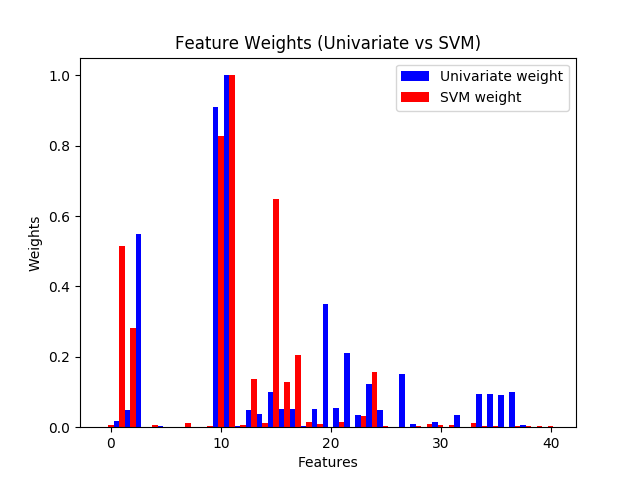
\includegraphics[width=1\textwidth]{images/ufe_svm.png}
	\caption{Weights assigned to the features by SVM and UFE} 
	\label{fig:result_ufe_svm}
\end{figure}

\subsection{Experiment 3}

After confirming the SVM feature ranks with that of UFE, we used Recursive Feature Elimination (RFE) with SVM and 10-fold cross-validation to remove weak features and calculate the accuracy. RFE iteratively eliminates one feature at a time and calculates the accuracy until just one feature remains.

\begin{figure}[htb]
	\centering
	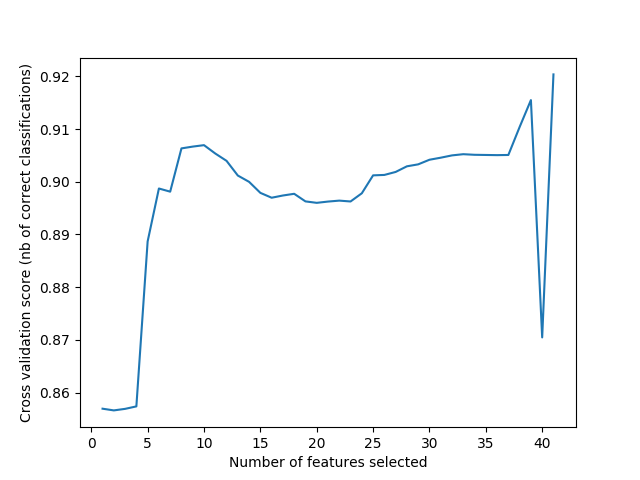
\includegraphics[width=1\textwidth]{images/rfe_svm.png}
	\caption{Recursive Feature Elimination with SVM} 
	\label{fig:result_rfe}
\end{figure}

As we can see from Figure \ref{fig:result_rfe}, we get within a $2$\% of the best result with just 6 features and within $1$\% with 10 features out of 41. It shows that the top 6 features in Table \ref{tab:5} contribute the most to the accuracy of the model.

\subsection{Experiment 4}

In this experiment we ran Random Forest Classifier with Recursive Feature Elimination and 10-fold cross-validation on the dataset to support the results given by SVM in previous section.

\begin{figure}[htb]
	\centering
	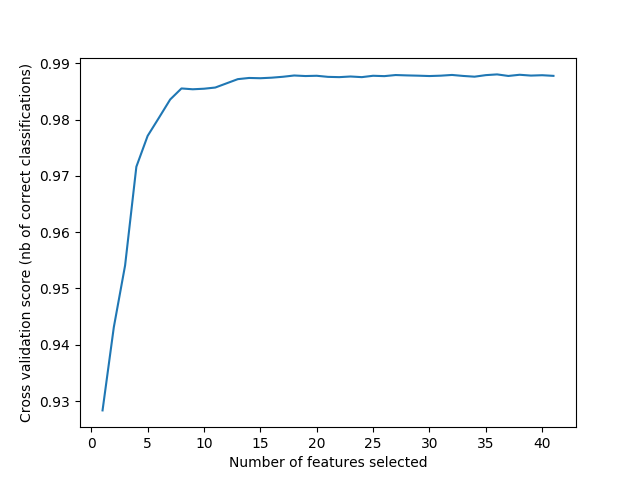
\includegraphics[width=1\textwidth]{images/rf_rfe.png}
	\caption{Recursive Feature Elimination with Random Forest} 
	\label{fig:result_rf_rfe}
\end{figure}

The first observation from Figure \ref{fig:result_rf_rfe} is that Random Forest gives us a much higher accuracy than SVM. It also supports the SVM result that the top 6 features contribute the most to the accuracy and the remaining features can be eliminated.

\subsection{Experiment 5}

In this experiment we ran XGBoost classifier with 10-fold cross validation and compared the results to that of SVM and Random Forest.

\begin{figure}[htb]
	\centering
	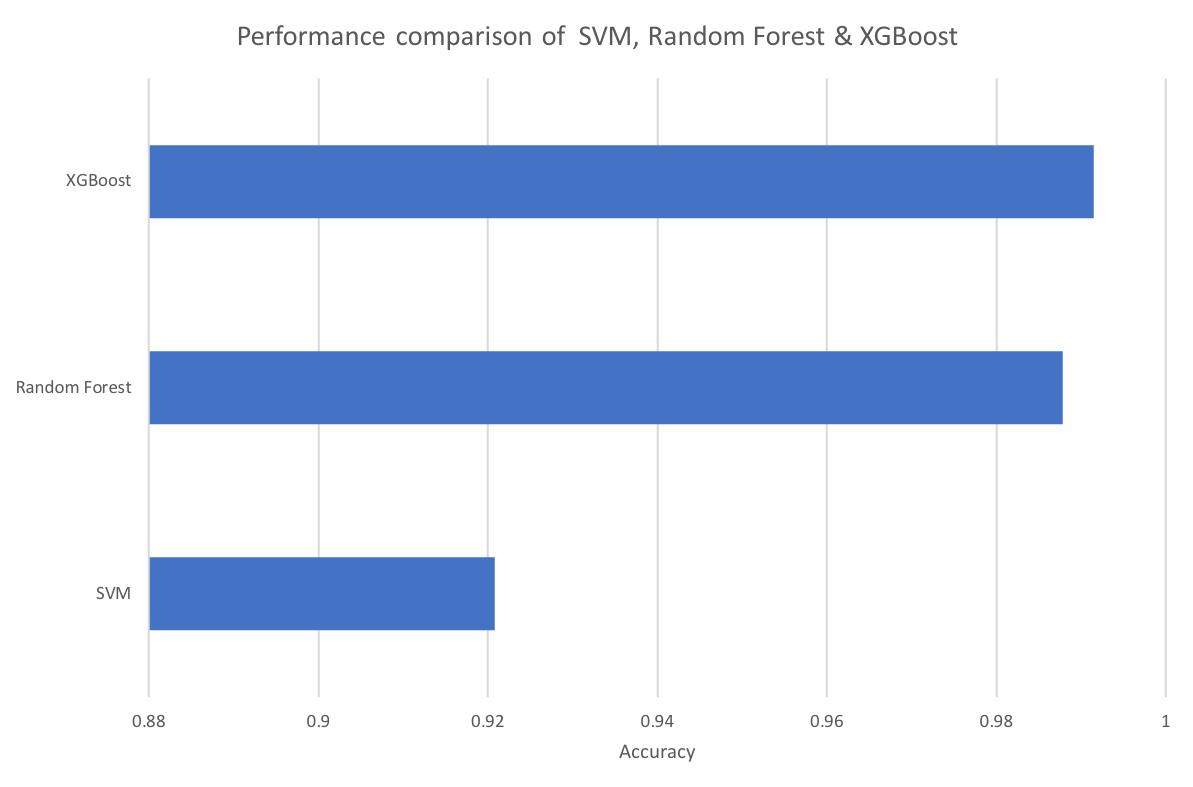
\includegraphics[width=1\textwidth]{images/svm_rf_xgb.png}
	\caption{Recursive Feature Elimination with Random Forest} 
	\label{fig:result_svm_rf_xgb}
\end{figure}

We can see that XGBoost gives us the highest accuracy of $99.15$\% followed by Random Forest which gives us an accuracy of $98.78$. Thus, we can say that ensemble techniques such as XGBoost and Random Forest performs the best on the given dataset and can be used to identify malicious encrypted traffic.